% !TeX encoding = UTF-8
% !TeX spellcheck = en_US
% !TeX root = main.tex

\chapter{Background and theory}
\label{sec:background}

\section{BESSY II}

\subsection{General presentation}
BESSY II (\textbf{B}erliner \textbf{E}lektronen\-\textbf{S}peicherring-Gesellschaft für \textbf{Sy}n\-chro\-tron\-strahlung m.b.H.) is Berlin electron storage ring, aimed at producing high energy light ray by synchrotron radiation. It emits extremely brillant photons pulse ranging from the long wave terahertz region to hard X rays, with an emphasis on the soft X-ray range~\cite{web:bessy_homepage}. Scientific projects can freely apply to an experimental station, where they are able to adjust the wavelength, polarization and photon energy. More than 2000 scientists per year are using BESSY II equipment.

The storage ring has a circumference of 240~meters and provides around 50 beamlines (paths of light rays between the accelerator and experimental stations). The electrons are accelerated to an energy up to 1.7~GeV.

BESSY II was inaugurated in 1998 and is since 2009 a facility of the \textit{Helmholtz-Zentrum Berlin für Materialien und Energie} (HZB), to study material structures and processes by guest scientists.

Additionally to the guest scientists, experts and operators\todo{I don't know how to call them} ensure the good functioning of the whole facility and work on refining the quality and the stability of the light rays. 

\subsection{General functioning}
The way BESSY II functions is based on the synchrotron radiation phenomenon: any accelerated particle emits radiations (in the form of photons), with a maximal amplitude in the case of a circular acceleration. \todo{Should I detail the equations?} It can be shown~\cite{book:wille} that the radiated power in circular acceleration can be given as 
\begin{equation}
P_s = \frac{e^2 c}{6 \pi \varepsilon_0}\frac{1}{(m_0 c^2)^4}\frac{E^4}{R^2}.
\end{equation}
where $c$ is the speed of light, $m_0$ the rest mass (independent of the velocity) of the particle, $e$ its charge, $E$ it's energy, $R$ the bending radius and $\varepsilon_0$ the  vacuum permittivity.

Considering their low mass, the electrons are very good candidates to produce high energy radiation.

The most important properties of the synchrotron radiation are its brilliance and brightness, which describe the quality of the beam. The brightness describes the angular divergence of the beam, and the brillance its transverse dimension: both are expected to be as small as possible to be in the configuration in which the beam is the most point-like. (See Section~\ref{sec:brightness_brillance} for the exact definitions).

The main purpose of BESSY II is to provide a light radiation with stable brilliance and brightness over time. To achieve this, the light source itself must be very stable as well. Therefore a significant attention is drawn to the control of the storage ring.
\begin{figure}
	\centering
	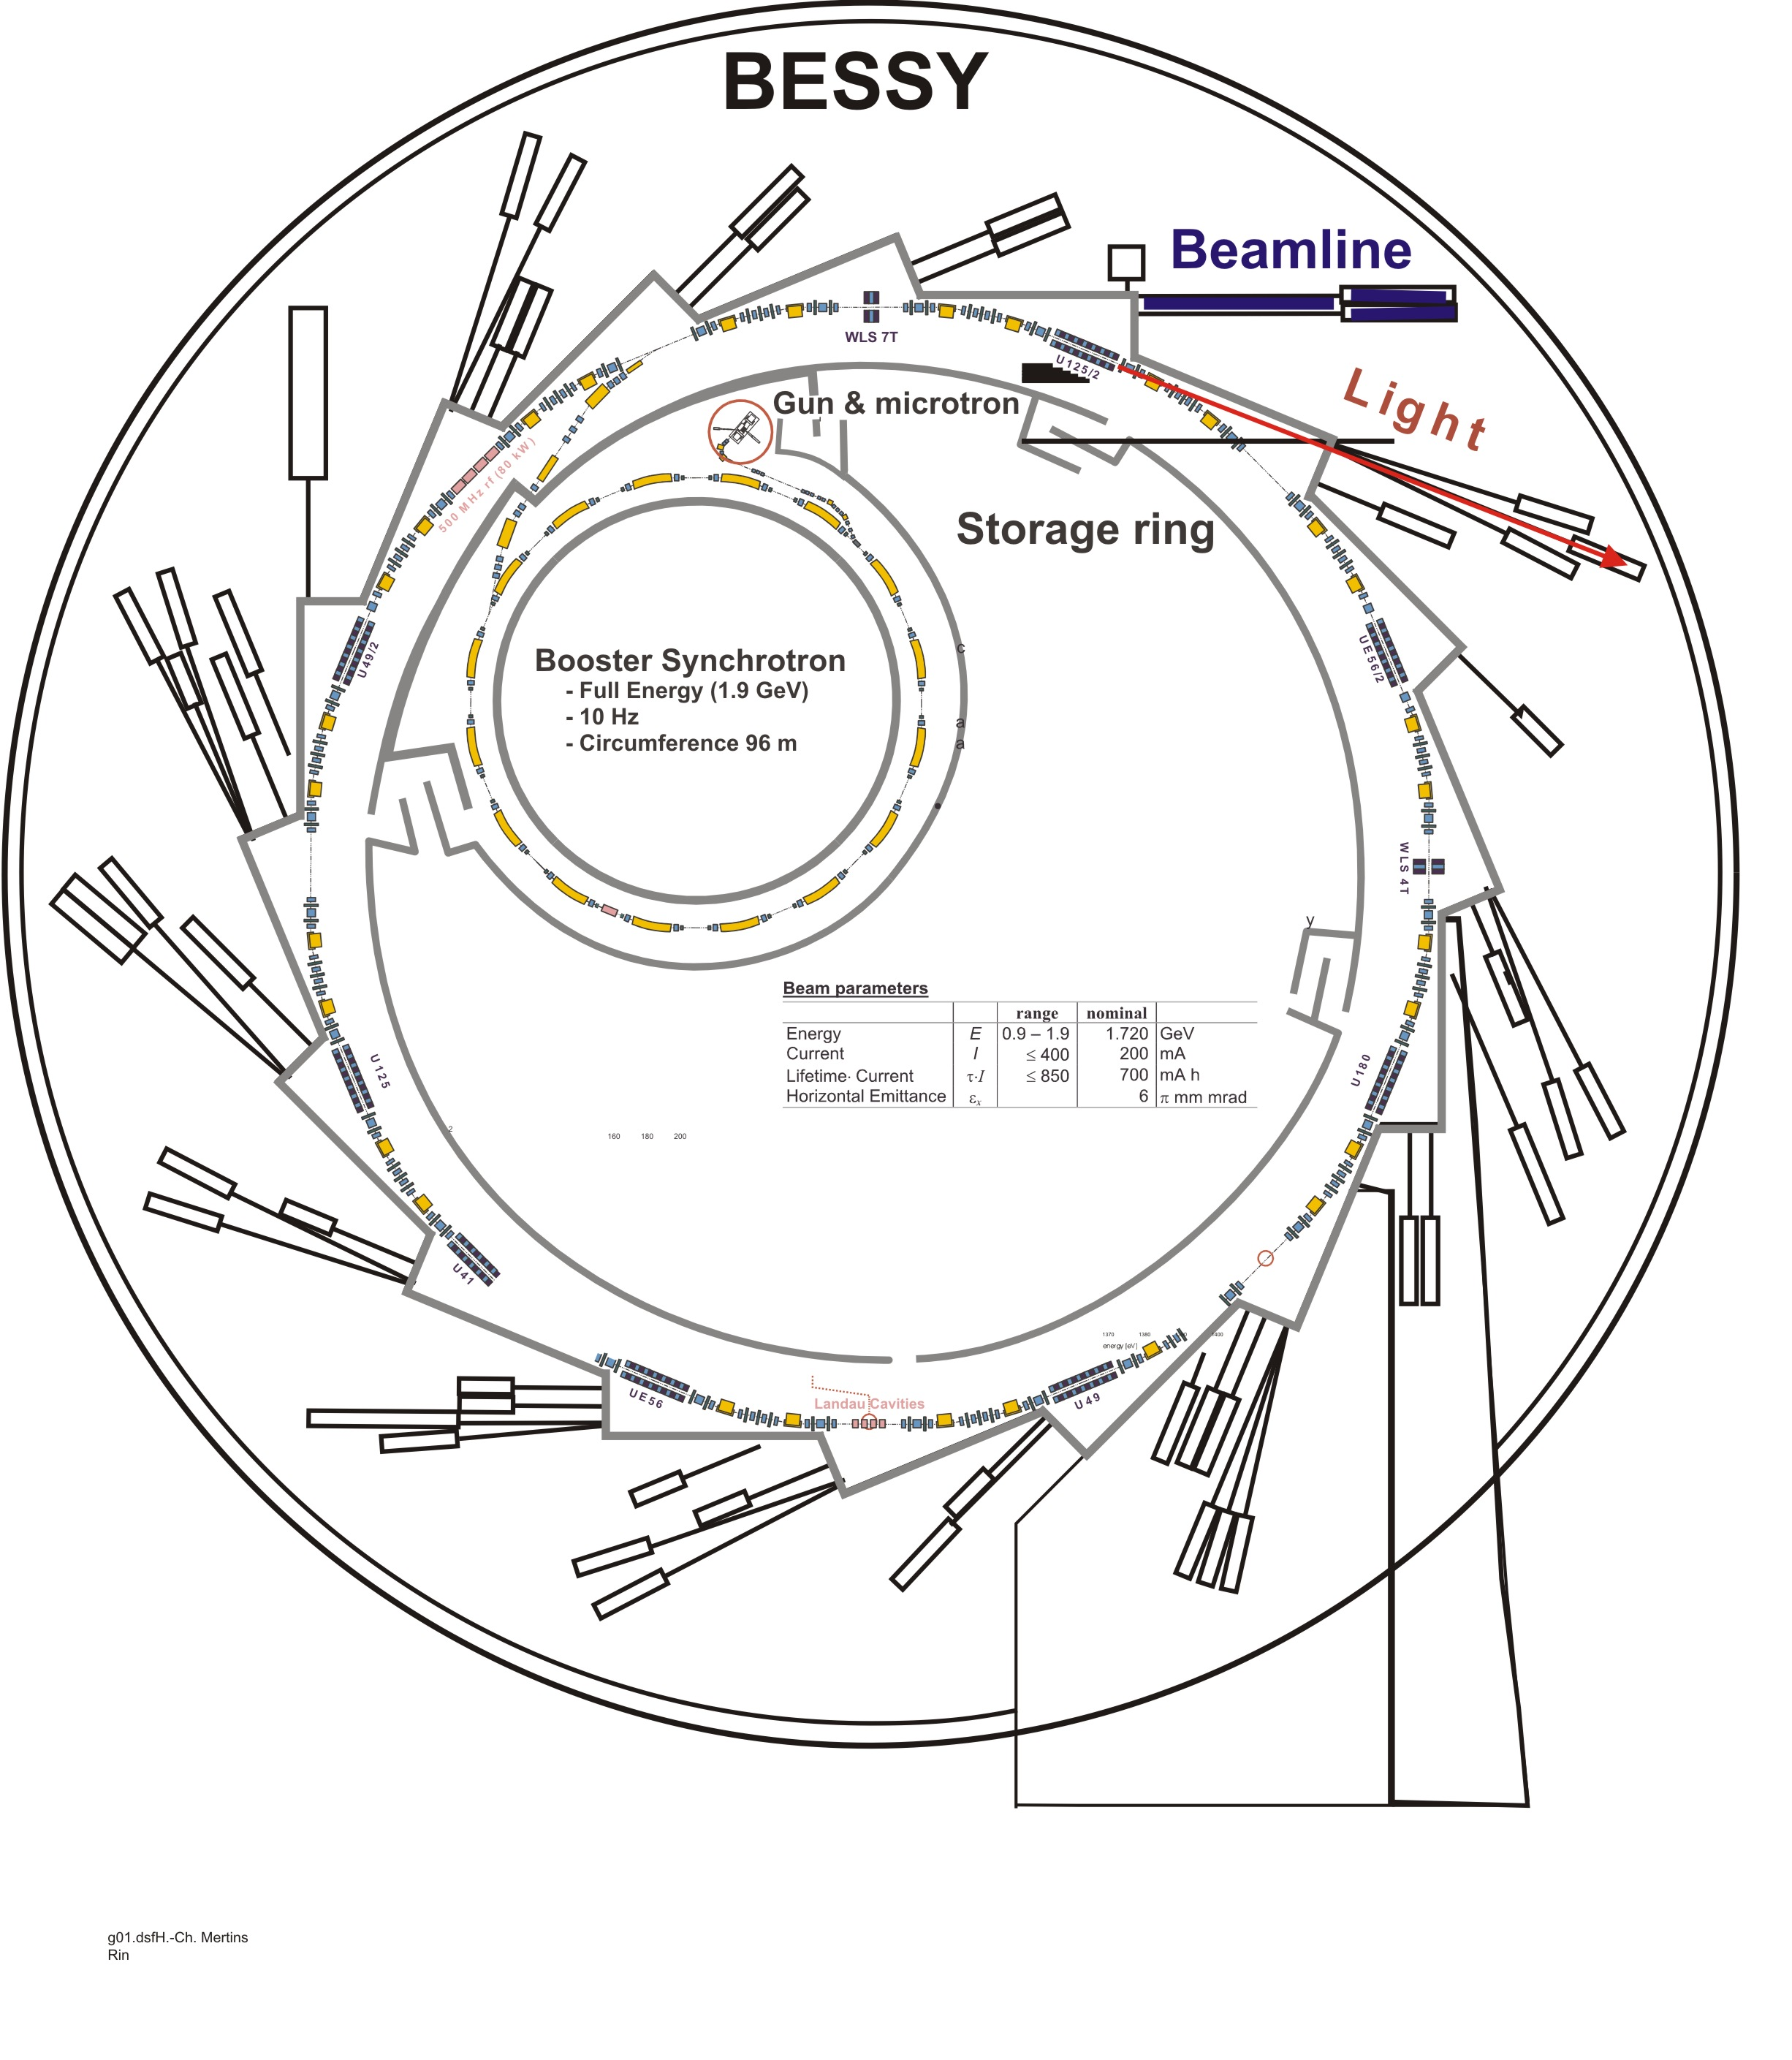
\includegraphics[width=0.8\textwidth]{img/bessy_acc_chain_web.jpg}
	\caption[Bessy II -- Accelerator chain]{\label{fig:bessy_acc_web_simple} Bessy II -- Accelerator chain (Source:~\cite{web:bessy_homepage})}
\end{figure}

\begin{sidewaysfigure}
    \centering
    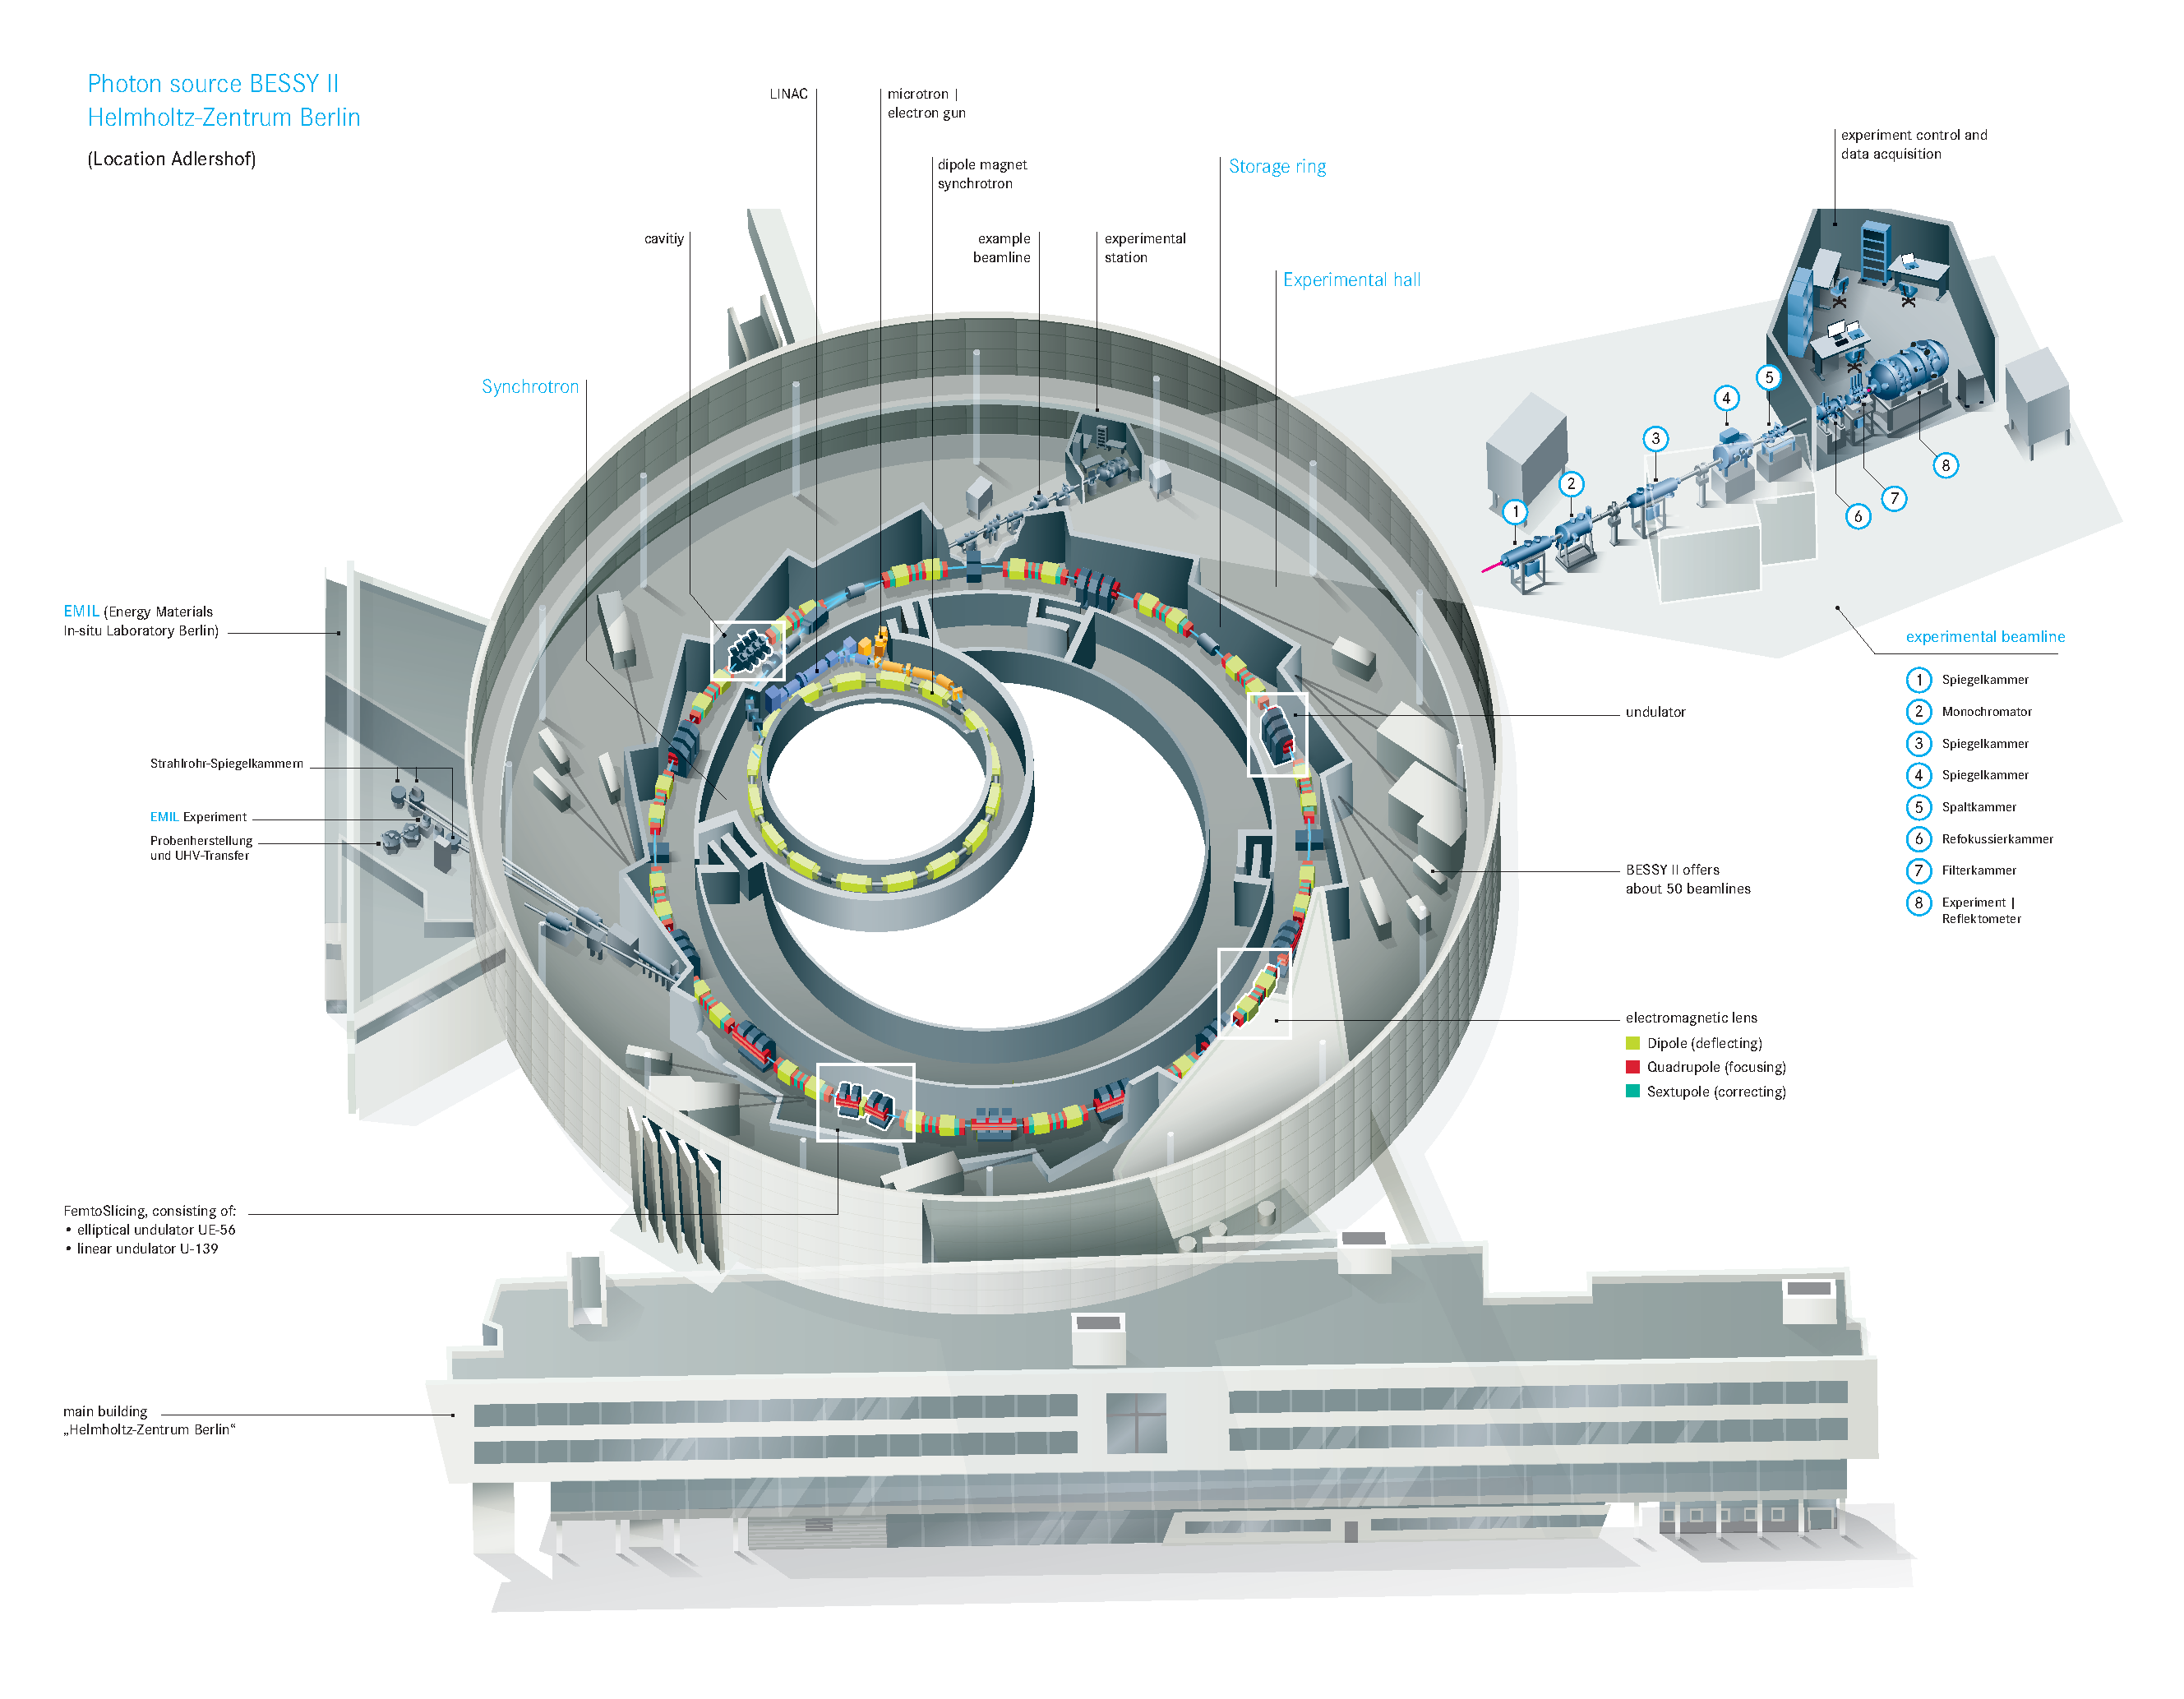
\includegraphics[width=0.8\textwidth,height=0.8\textheight,keepaspectratio]{img/bessy_acc_web.pdf}
    \caption[Bessy II facility]{\label{fig:bessy_acc_web} Bessy II facility (Source:~\cite{web:bessy_homepage})}
\end{sidewaysfigure}

In order to reach an energy of 1.7~GeV, the electrons undergo several chained accelerations (see \autoref{fig:bessy_acc_web}), namely:\todo{energies}
\begin{enumerate}
    \item an electron canon gives the electrons their first impulse
    \item a microtron accelerate them to an energy of XXX
    \item a LINAC (\textbf{lin}ear \textbf{ac}celerator) increase the energy to XXX
    \item the booster (a synchrotron) give them the final energy of XXX.
\end{enumerate}

When this energy is reached, the electrons are injected to the storage ring, which ensure that the electrons are kept at the same energy.

Because of the synchrotron radiation, the bunches of particles lose regularly their energy; therefore a new injections from the accelerations chain take place every XXX\todo{time} to repopulate the storage ring and stabilize its energy.

\section{Particle accelerator physics}
In order to understand the trajectory perturbations, the basic physics of the particle accelerator must be addressed.

\subsection{Synchrotron basics}
To study the beam trajectory, one possibility is to use the linear beam optics (by analogy between beam and light focusing and steering). We solely describe here what is needed in the next sections. A full reference can be found in~\cite{book:wille}. This section is mostly inspired by the chapter 3 of this same reference.

\subsubsection{Geometry -- Frame of reference -- Kinematics}
The term \emph{orbit} refers to the ideal trajectory of the particles, which is fixed by the construction of the accelerator.

The frame of reference is $K=(\vec{e}_x,\vec{e}_y, \vec{e}_s)$, which origin follows the beam. $\vec{e}_x$ is the horizontal axis directed towards the exterior of the orbit and normal to its curve, $\vec{e}_y$ is the vertical axis and $\vec{e}_s$ the tangential axis to the orbit.
\begin{figure}[!h]
    \centering
    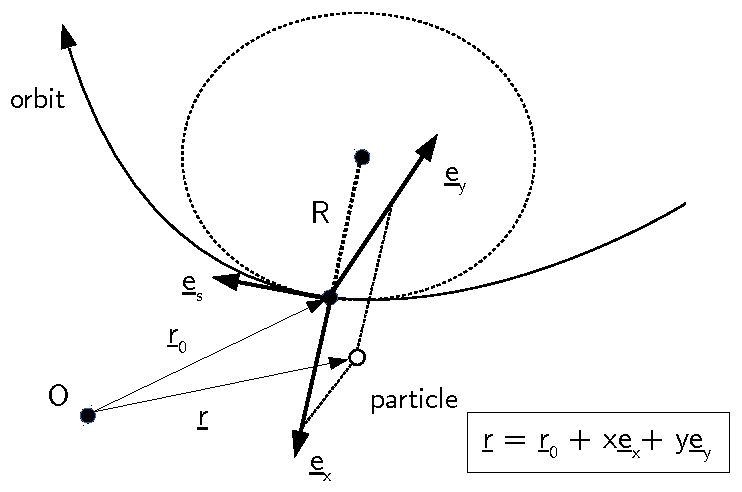
\includegraphics[width=0.8\linewidth]{img/orbit_coordinates.pdf}
    \caption{\label{fig:coordinate system}Description of the co-moving coordinate system}
\end{figure}
Let $\varphi$ be the azimuth angle, oriented by $\vec{e}_y$. Then, since $ds = -R d\varphi$, we can write
\begin{equation}
\frac{d \varphi}{d t}  = -\frac{1}{R} \frac{d s}{d t}.
\end{equation}

Using the derivation formula of polar coordinate we can write:
\begin{align}
&\dot{\vec{e}}_x = \frac{d\vec{e}_x}{d t} = -\dot{\varphi} \vec{e}_s = \frac{1}{R} \dot{s}\vec{e}_s \nonumber \\
&\dot{\vec{e}}_y = 0 \\
&\dot{\vec{e}}_s = \frac{d\vec{e}_s}{d t} = \dot{\varphi} \vec{e}_x = -\frac{1}{R} \dot{s}\vec{e}_x \nonumber.
\end{align}

Let $\vec{r} = \vec{r}_0 + x\vec{e}_x + y \vec{e}_y$ be the position of a given particle in a Galilean reference frame (with $\vec{r}_0$ the position of the origin of the moving coordinates, see Fig.~\ref{fig:coordinate system}) and let's define $x'$ the spatial derivative with respect to $s$ so that:
\begin{equation}
\begin{aligned}
&\dot{x}= \frac{dx}{ds}\frac{ds}{dt} = x'\dot{s}  \\
&\ddot{x}= x''\dot{s}^2+x'\ddot{s}.
\end{aligned}
\end{equation}
It follows, after some algebraic manipulations:
\begin{align}
\label{eq:kinematics}
&\vec{r} = \vec{r}_0 + x\vec{e}_x + y \vec{e}_y \nonumber \\
&\dot{\vec{r}}= x' \dot{s} \vec{e}_x + y'\dot{s} \vec{e}_y  + \left(1+\frac{x}{R}\right)\dot{s}\vec{e}_s\\
&\ddot{\vec{r}}= \left[x'' \dot{s}^2 + x' \ddot{s} - \left( 1+\frac{x}{R} \right)\frac{\dot{s}^2}{R}\right] \vec{e}_x + (y''\dot{s}^2 + y'\ddot{s}) \vec{e}_y \nonumber \\
& \hspace{14em} + \left[\frac{2}{R}x'\dot{s}^2 +\left(1+\frac{x}{R}\right)\ddot{s}\right]\vec{e}_s \nonumber
\end{align}

\subsubsection{Hypotheses} We assume the following hypotheses are valid.
\begin{description}
    \item{H1 --} The particles move essentially parallel to $\vec{e}_s$: in the first order
    \begin{equation*}
        \vec{v} = v_s \vec{e}_s.
    \end{equation*}
    \item{H2 --} The magnetic field has only transverse components:
        \begin{equation*}
        \vec{B} = (B_x, B_y, 0)
        \end{equation*}
    \item{H3 --} The electric field is negligible with respect to the magnetic field.
    \item{H4 --} The velocity of the particle varies very slowly in a magnet: $\ddot{s} \approx 0$
    \item{H5 --} The particles move at relativistic velocities, so the effect of the magnetic field is negligible on longitudinal components: we consider only transverse components.
    \item{H6 --} The momentum of the particles is $p = p_0+\Delta p$, with the condition $\Delta p \ll p_0$ (which is well satisfied in accelerators).
\end{description}

\subsubsection{Equation of motion}
Newton's second law can be applied with the Lorentz force:
\begin{equation}
\dot{\vec{p}} = e(\vec{E}+\vec{v} \times \vec{B}) 
\end{equation}
which according to (H3) becomes
\begin{equation}
\ddot{\vec{r}} = \frac{e}{m}(\dot{\vec{r}} \times \vec{B})
\end{equation}

According to (H2), the magnetic field is only transversal, which yields:
\begin{equation}
\label{eq:lorentz_transv}
\ddot{\vec{r}} = \frac{e}{m}(\dot{\vec{r}} \times \vec{B})
= \frac{e}{m}
    \begin{pmatrix}
        -\left(1+\frac{x}{R}\right)\dot{s}B_y \\
        \left(1+\frac{x}{R}\right)\dot{s}B_x \\
        x'\dot{s}B_y - y'\dot{s}B_x
    \end{pmatrix}.
\end{equation}

Using (H5), we can focus on the x- and y-components, (H4) in Eq.~\eqref{eq:kinematics} allow us to remove every $\ddot{s}$ factors, so that Eq.~\eqref{eq:lorentz_transv} can be rewritten as
\begin{equation}
\begin{aligned}
x'' \dot{s}^2 - \left(1+\frac{x}{R}\right)\frac{\dot{s}^2}{R}
&= -\frac{e}{m} \left(1+\frac{x}{R}\right)\dot{s}B_y \\
y'' \dot{s}^2 &=    \left(1+\frac{x}{R}\right)\dot{s}B_x.
\end{aligned}
\end{equation}
Finally, because $p=mv$ and using Eq.~\eqref{eq:kinematics} combined with (H1), we can replace
\begin{equation}
m = \frac{p}{v} = \frac{p}{\scal{\vec{v}}{\vec{e}_s}} = \frac{p}{\left(1+\frac{x}{R}\right)\dot{s}}
\end{equation}
to obtain:
\begin{equation}
\begin{aligned}
x''-\left(1+\frac{x}{R}\right)\frac{1}{R} &= -\frac{e}{p} B_y\left(1+\frac{x}{R}\right)^2 \\
y'' &= \frac{e}{p} B_x\left(1+\frac{x}{R}\right)^2
\end{aligned}
\end{equation}

(H6) allow us to write, to first order:

\begin{equation*}
\frac{1}{p} = \frac{1}{p_0} \left(1-\frac{\Delta p}{p_0}\right).
\end{equation*}

Furthermore the magnetic field can be approximated to first order with:
\begin{equation}
\frac{e}{p_0} B_y = \frac{1}{R}-kx \qquad\qquad \frac{e}{p_0} B_x = -ky
\end{equation}
which yields
\begin{equation}
\begin{aligned}
x''-\left(1+\frac{x}{R}\right)\frac{1}{R} &= -\left(\frac{1}{R}-kx\right)\left(1-\frac{\Delta p}{p_0}\right)\left(1+\frac{x}{R}\right)^2 \\
y'' &= -ky\left(1-\frac{\Delta p}{p_0}\right)\left(1+\frac{x}{R}\right)^2
\end{aligned}
\end{equation}

Finally by removing terms of second order ($\frac{x}{R} \ll 1$, $\frac{\Delta p}{p_0} \ll 1$) we obtain the linear equations of motion in a magnetic structure:

\begin{empheq}[box=\fbox]{equation}
\label{eq:motion_particle}
\begin{aligned}
x''(s) + \left(\frac{1}{R^2(s)} - k(s)\right) x(s) &= \frac{1}{R(s)}\frac{\Delta p}{p_0} \\
y''(s) + k(s) y(s) &= 0
\end{aligned}
\end{empheq}

\subsubsection{Beta function and betatron oscillation}

The beta function will provide a description of properties of a beam of many particles.

We use \ref{eq:motion_particle} and only assume that $\frac{1}{R} = 0$ and $\frac{\Delta p}{p_0}=0$. The orbit curve is thus assumed almost flat and the momentum deviation negligible. We obtain Hill's differential equation: 

\begin{equation}
\label{eq:hill_diff}
	x''(s) - k(s) x(s) = 0
\end{equation}
which solution is the transverse oscillation of the orbit, or \emph{betatron oscillation}

\begin{equation}
\label{eq:hill_sol_cst}
x(s) = A u(s) \cos \left(\Psi(s)+\phi \right).
\end{equation}

The phase and the amplitude depend of the position $s$; $A$ and $\phi$ being integration constants.

By inserting \eqref{eq:hill_sol_cst} in \eqref{eq:hill_diff} we obtain
\begin{equation}
A\left[u''- u \Psi'^2 - k u \right] \cos\left(\Psi+\phi\right) - A\left[2u'\Psi'+u\Psi''\right]\sin\left(\Psi+\phi\right) = 0.
\end{equation}

$A \ne 0$ and $\Psi(s)$ having different values for every $s$, the previous equation yields:
\begin{align}
u''- u \Psi'^2 - k u = 0 \label{eq:hill_cond1}\\
2u'\Psi'+u\Psi'' = 0 \label{eq:hill_cond2}
\end{align}

Eq. \eqref{eq:hill_cond2} leads to:
\begin{equation}
2\frac{u'}{u} + \frac{\Psi''}{\Psi'} = 0
\end{equation}
which can be integrated as
\begin{equation}
\label{eq:phase_psi}
\Psi(s) = \int \limits_{0}^{s} \frac{d\sigma}{u^2(\sigma)}.
\end{equation}

%By inserting this result into \eqref{eq:hill_cond1} we obtain
%\begin{equation}
%u'' - \frac{1}{u^3} - k u = 0
%\end{equation}

The \emph{beta function} $\beta(s)$ is defined as
\begin{equation}
\label{eq:beta_func}
\beta(s) := u^2(s)
\end{equation}

By substituting $A = \sqrt{\varepsilon}$, we obtain the final trajectory equation
\begin{empheq}[box=\fbox]{equation}
	\label{eq:orbit_equation}
	x(s) = \sqrt{\varepsilon \beta(s)} \cos\left(\Psi(s)+\phi \right)
\end{empheq}

$\varepsilon$ is a constant termed \emph{emittance} and the envelop of the orbit at each position $s$ is $E(s) = \sqrt{\varepsilon \beta(s)}$, which defines the size of the beam.

\remark The calculation done for the $x$ direction can be done similarly for the $z$ one.

\remark Since the beta function controls the size of the beam, it must be finely controlled. A matrix calculation method is presented in \cite{book:wille} in order to calculate it step by step around the orbit. Knowing this, $\Psi$ can be calculated by rewriting Eq.~\eqref{eq:phase_psi} as 
\begin{equation}
\Psi(s)=\int \limits_{0}^{s} \frac{d\sigma}{\beta(\sigma)},
\end{equation}
and the particle trajectories can be calculated for a given emittance.

\subsubsection{Brightness and brilliance}
\label{sec:brightness_brillance}
In the following section, the $\theta$ subscript is either $x$ or $z$.

We first define the \emph{flux} F of photons, normalized to a beam current of 1~A:
\begin{equation}
F = \frac{\text{photons}}{\text{s 0.1\% BW A}}
\end{equation}

To describe the quality of the beam, which the \emph{brightness} and the \emph{brilliance} are defined.

The brightness describes the angular divergence of the beam (given by $\sigma_\theta'=\sqrt{\frac{\varepsilon_\theta}{\beta_\theta}}$). It is defined as:
\begin{equation}
S = \frac{F}{2 \pi \sigma'_x \sigma'_z} = \frac{F \sqrt{\beta_x \beta_z}}{2 \pi \sqrt{\varepsilon_x \varepsilon_z}} = \frac{\text{photons}}{\text{s 0.1\% BW mrad$^2$ A}}
\end{equation}
while the brilliance relates to the transverse dimensions ($\sigma_\theta=\sqrt{\varepsilon_\theta \beta_\theta}$):
\begin{equation}
B = \frac{F}{4 \pi^2 \sigma_x \sigma_z \sigma'_x \sigma'_z} = \frac{F}{4 \pi^2 \varepsilon_x \varepsilon_z} = \frac{\text{photons}}{\text{s 0.1\% mm$^2$ BW mrad$^2$ A}}
\end{equation}
These definitions vary in literature. These are taken from the book of K.~Wille~\cite{book:wille}, and apply to Gaussian-shaped electron beams. The invariant idea is that both values are determinated by the beam emittance $\sigma$: the design of the accelerators and the correction are aimed at obtaining the smallest emittance $\varepsilon_\theta$ as possible.

\subsubsection{Tune}


\subsection{Booster and storage ring}
\todo[inline]{What is particular in storage ring}
Both the booster and the storage ring are synchrotrons. The former aims at accelerating the particles, whereas the latter aims at storing them with a constant energy. 

\section{Orbit and distortions}
\todo[inline]{Physics + examples = 1/2 - 1 pges}
\subsection{Theory}
The accelerators are designed so that the particles follow a given path, which is defined in the case of synchrotrons by the successive bendings involved by the magnets. As the precision of the positioning of the magnets is limited, some errors may destabilize the orbit and increase the dispersion of the particles around the theoretical orbit. In addition, the environment produces perturbations: for instance the 50~Hz of the main power, some not perfectly isolated magnetic sources.

In order not to lose electrons in the walls of the vacuum chamber but also to increase the brightness of the synchrotron radiations (and therefore to have focused electron beams), all these residual misalignment and magnetic field errors must be corrected.

\subsection{Distortions in BESSY II}


